\documentclass[11pt]{report}
\usepackage{mathtools}
\usepackage{amsmath}
\usepackage{amssymb}
\usepackage{amsfonts}
\usepackage{amsthm}
\usepackage{xcolor}
\usepackage{graphicx}
\usepackage[top=2.0cm,bottom=2.0cm,left=2.5cm,right=2.5cm]{geometry}
\usepackage{tikz}
\usepackage{float}
\usepackage{multicol}
\usepackage{pgfplots}
\usepackage{lastpage}
\usepackage{siunitx}
\usepackage{xspace}
\usepackage[labelfont=bf]{caption}
\usepackage[hidelinks, urlcolor=blue, linkcolor=blue, colorlinks=true]{hyperref}
\usepackage[capitalize,noabbrev]{cleveref}
\usepackage[absolute]{textpos}
\usepackage{systeme}

\newcommand{\R}{\mathbb{R}}
\newcommand{\C}{\mathbb{C}}
%% define course title
\newcommand{\course}{MAT185}
\newcommand{\assignmenttitle}{Assignment 1}

%% header and footer
\firstpageheader{}{}{\textbf{{\color{red} Due:} 10:00pm, Tuesday Jan. 21, 2025}}
\firstpageheadrule
\runningheader{}{Page~\thepage~of~\numpages}{\course~--~\assignmenttitle}
\footer{}{}{}

\setlength\parindent{0pt} % no indentation in document

%% formats exam class
\qformat{\textbf{Question \thequestiontitle:}\hfill} % title of question 
\boxedpoints
\pointpoints{mark}{marks}
\pointsinrightmargin
\hpword{Marks:}
\hsword{Your score:}
\unframedsolutions
\totalformat{\boxed{\textnormal{\totalpoints~\if\totalpoints1 mark\else marks\fi}}}
\definecolor{SolutionColor}{rgb}{0,0,1}
\renewcommand{\solutiontitle}{}
\AtBeginEnvironment{solution}{\color{blue}}

% %correct choices in solution
\CorrectChoiceEmphasis{\rm}
\checkedchar{\tikz\draw[blue,fill=blue] (0,0) circle (1ex);}

% % increase distance between checkbox items
\renewcommand{\checkboxeshook}{\setlength{\itemsep}{6pt}}

%% distance between questions and parts
\renewcommand{\questionshook}{\setlength{\parsep}{10pt}}
\renewcommand{\partshook}{\setlength{\parsep}{15pt}}

%% define arrows in text
\newcommand{\arrow}{$\rightarrow$\xspace}
\newcommand{\Arrow}{$\Rightarrow$\xspace}

% % math notation:
%\veccol{1}{2}{3}
\newcommand{\veccol}[3]{
    \begin{bmatrix}
        #1\\
        #2\\
        #3\\
    \end{bmatrix}}
  
%\vecrow{1}{2}{3}
\newcommand{\vecrow}[3]{\left[#1~#2~ #3\right]}

%\matrixTwo{1}{2}{3}{4}
\newcommand{\matrixTwo}[4]{\left[\begin{array}{cc}#1&#2\\#3&#4\end{array}\right]}

% \matrixThree{1}{2}{3}{4}{5}{6}{7}{8}{9}
\newcommand{\matrixThree}[9]{\left[\begin{array}{ccc}#1&#2&#3\\#4&#5&#6\\#7&#8&#9\end{array}\right]}

%\matrixCorner{1}{2}{3}{4}
\newcommand{\matrixCorner}[4]{\left[\begin{array}{ccc}#1& \cdots&#2\\ \vdots & \ddots & \vdots\\#3&
      \cdots&#4\end{array}\right]}

% \nR
\newcommand{\nR}{{}^{n}\mathbb{R}}
% \Rn
\newcommand{\Rn}{\mathbb{R}^{n}}
% \nRn
\newcommand{\nRn}{{}^{n}\mathbb{R}^{n}}
% \nRm
\newcommand{\nRm}{{}^{n}\mathbb{R}^{m}}
% \nRm
\newcommand{\mRn}{{}^{m}\mathbb{R}^{n}}
% \mRm
\newcommand{\mRm}{{}^{m}\mathbb{R}^{m}}        

% \u
\renewcommand{\u}{{\bf u}}      
% \v
\renewcommand{\v}{{\bf v}}      
% \w
\newcommand{\w}{{\bf w}}    
% \V
\newcommand{\V}{{\bf V}}                   
       
%% define abbreviations
\newcommand{\row}{\operatorname{row}\,}
\newcommand{\col}{\operatorname{col}\,}
\renewcommand{\dim}{\operatorname{dim}\,}
\renewcommand{\span}{\operatorname{span}\,}
\newcommand{\rank}{\operatorname{rank}\,}
\renewcommand{\ker}{\operatorname{ker}\,}
\newcommand{\nul}{\operatorname{null}\,}
\renewcommand{\det}{\operatorname{det}\,}
\newcommand{\adj}{\operatorname{adj}\,}

\usepackage{xcolor}
% Sean's original colours:
%\definecolor{dkrgreen}{rgb}{0.1, 0.4, 0.3} 
\definecolor{dkrgreen}{HTML}{009988} % this is the color-blind friendly teal from below
%\definecolor{dkred}{rgb}{0.8, 0.05, 0.05} 
\definecolor{dkred}{HTML}{EE3377}  % this is the colour-blind friendly magenta from below
%\definecolor{orange}{rgb}{0.8, 0.33, 0.0}
%\definecolor{goldenrod}{rgb}{0.85, 0.65, 0.13}
\definecolor{blue}{HTML}{1965B0} % this is the colour-blind friendly blue from below
%
% colour-blind-friendly colours from https://personal.sron.nl/~pault/
\definecolor{tolBlue}{HTML}{1965B0}
\definecolor{tolMedBlue}{HTML}{5289C7}
\definecolor{tolLightBlue}{HTML}{7BAFDE} 
\definecolor{tolRed}{HTML}{E8601C} 
\definecolor{tolYellow}{HTML}{F6C141}
\definecolor{tolTeal}{HTML}{009988}
%\definecolor{tolBlue}{HTML}{0077BB} 
\definecolor{tolCyan}{HTML}{33BBEE}
\definecolor{tolTeal}{HTML}{009988} 
\definecolor{tolOrange}{HTML}{EE7733} 
%\definecolor{tolRed}{HTML}{CC3311} 
\definecolor{tolMagenta}{HTML}{EE3377} 
\definecolor{tolGrey}{HTML}{BBBBBB}

%%% This command makes a framed box of a chosen height.
\newcommand{\makenonemptybox}[2]{%
\par\nobreak\vspace{\ht\strutbox}\noindent
\setlength{\fboxrule}{0pt} % set this to 0pt to make invisible
\fbox{%
\parbox[c][#1][t]{\dimexpr\linewidth-2\fboxsep}{
  \hrule width \hsize height 0pt
  \vspace{-0.6cm}
  \color{SolutionColor}#2\color{black}
 }%
}%
}


\begin{document}
\thispagestyle{empty}
{\LARGE \bf ECE 253 Lecture Notes}\\
{\large Hei Shing Cheung}\\
Digital and Computer Systems, Fall 2025 \hfill ECE253\\
\\
The up-to-date version of this document can be found at \url{https://github.com/HaysonC/skulenotes}\\

\chapter{Digital Circuits that Compute, Store, and Control}
\begin{shaded}
\section*{Introduction}
\paragraph{Layers of Computation} In hardware, we have the following layers of abstraction:
\begin{itemize}
    \item Computation
    \item Adders 
    \item Logic Gates
    \item Transistors
    \item Silicon
\end{itemize}
In this course, we will focus on the first three layers, on top of the logic gate level.


\paragraph{Layer of abstraction} At this course, for the digital systems part, we would start from understanding logic gates, all the way to understanding computer architecture, with each level of abstraction hiding the details of the lower level.

\subsection{Hierarchy, Modularity, and Regularity}

\begin{definition}[Hierarchy]
    The division of system into a set of modules, then further subdividing each module into smaller modules, and so on, until pieces are \textit{easy} to understand.    
\end{definition}

\begin{definition}[Modularity]
    The design principle that modules have well-defined functions and interfaces so they connect easily without unintended side effects.
\end{definition}

\begin{definition}[Regularity]
    The uniformality of modules, such that the reusability of common modules reduces the number of distinct modules to be designed.
\end{definition}

\subsection{Digital Logic Gates}
Logic gates are made out of transistors:
\begin{definition}[Transistor]
    A transistor is a 3-terminal device behaving as a switch. When the voltage on the terminal is HI, the switch is closed, and when the voltage is LO, the switch is open.
\end{definition}

\paragraph{Factors Affecting Speed of Digital Circuits}
\begin{itemize}
    \item \textbf{Transistors and Electrons take time to switch.} A transistor (State of the Art) takes 2-3 picoseconds to switch. Gates takes 40 ps and an 8-bit adder takes 300 ps.
    \item \textbf{Wires take time to propagate signals.} Signals travel at approximately 2/3 the speed of light in a vacuum, which is about 200,000 kilometers per second in a typical silicon wire.
    \item \textbf{Capacitance} There would be RCL circuits formed by the wires and transistors, which would cause delay.
\end{itemize}

\end{shaded}

\section{Logic Circuits}
\subsection{Number Systems}
\begin{definition}[Number System]
    A number system is a way of representing numbers using a set of symbols (digits) and a base (radix). The base determines the number of unique digits that can be used in the number system.
\end{definition}

\paragraph{Common Number Systems} You should be familiar with the following number systems:
\begin{itemize}
    \item Decimal (Base 10): Digits 0-9
    \item Binary (Base 2): Digits 0-1
    \item Hexadecimal (Base 16): Digits 0-9, A-F
\end{itemize}

In computer systems, we use binary to represent information, and we would often use hexadecimal to represent binary numbers in a more compact way - a group of 4 bits (a nibble) can be represented by a single hexadecimal digit.

\begin{example}[Binary, Decimal, and Hexadecimal Numbers]
    Below is a table showing the conversion of binary numbers to decimal numbers, along with their hexadecimal representation.
    \begin{table}[h!]
        \centering
        \begin{tabular}{|c|c|c|}
            \hline
            Binary & Decimal & Hexadecimal \\
            \hline
            0000 & 0 & 0 \\
            0001 & 1 & 1 \\
            0010 & 2 & 2 \\
            0011 & 3 & 3 \\
            0100 & 4 & 4 \\
            0101 & 5 & 5 \\
            0110 & 6 & 6 \\
            0111 & 7 & 7 \\
            1000 & 8 & 8 \\
            1001 & 9 & 9 \\
            1010 & 10 & A \\
            1011 & 11 & B \\
            1100 & 12 & C \\
            1101 & 13 & D \\
            1110 & 14 & E \\
            1111 & 15 & F \\
            \hline
        \end{tabular}
        \caption{Binary to Decimal and Hexadecimal Conversion}
    \end{table}
    
\end{example}
\begin{example}[Decimal to Binary Conversion]
    To convert a decimal number to binary, we can use the method of successive division by 2. For example, to convert the decimal number 437 to binary:
    \begin{align*}
        437 \div 2 &= 218 & \text{remainder 1} \\
        218 \div 2 &= 109 & \text{remainder 0} \\
        109 \div 2 &= 54 & \text{remainder 1} \\
        54 \div 2 &= 27 & \text{remainder 0} \\
        27 \div 2 &= 13 & \text{remainder 1} \\
        13 \div 2 &= 6 & \text{remainder 1} \\
        6 \div 2 &= 3 & \text{remainder 0} \\
        3 \div 2 &= 1 & \text{remainder 1} \\
        1 \div 2 &= 0 & \text{remainder 1}
    \end{align*}
    Reading the remainders from bottom to top, we get the binary representation of 437
\end{example}

\begin{example}
    To convert (512000)$_{10}$ to binary, we recognize that $512000 = 2^9 \times 1000$. We know that $2^9 = 512$ and $1000_{10} = 1111101000_2$ (by method outlined above). Therefore, we can shift the binary representation of 1000 left by 9 bits to get the binary representation of 512000:
    \[(512000)_{10} = (1111101000000000000)_2\]
\end{example}

\paragraph{Note} An alternative method is to devide by powers of 2.
\begin{shaded}
    \textbf{Fractional Numbers. } To represent fractional numbers in binary, we can use the method of successive multiplication by 2 (fixed point representation). Or we can use floating point representation, which is similar to scientific notation in decimal. 
\end{shaded}
\subsection{Binary Arithmetic and Logic}
\paragraph{Binary Arithmetic} Binary arithmetic is similar to decimal arithmetic, but it only uses two digits (0 and 1). Addition is associated with a sum and carry.

\paragraph{Binary Addition} The rules for binary addition are as follows: \\
\begin{table}[h!]
    \centering
    \begin{tabular}{|c|c|c|}
        \hline
        A & B & Sum, Carry \\
        \hline
        0 & 0 & 0, 0 \\
        0 & 1 & 1, 0 \\
        1 & 0 & 1, 0 \\
        1 & 1 & 0, 1 \\
        \hline
    \end{tabular}
    \caption{Binary Addition}
\end{table}

This could be summerize as the following logic:
\begin{equation}
    \text{Sum} = A \oplus B, \quad \text{Carry} = A \cdot B
\end{equation}
\paragraph{Binary Subtraction} The rules for binary subtraction are defined using the addition of negative numbers (2's complement):

\begin{definition}[Least Significant Bit (LSB) and Most Significant Bit (MSB)]
    The least significant bit (LSB) is the rightmost bit in a binary number, while the most significant bit (MSB) is the leftmost bit.`'
    
\end{definition}
\begin{definition}[2's Complement]
    The 2's complement of a binary number is obtained by inverting all the bits (1's complement) and adding 1 to the least significant bit (LSB).
\end{definition}

\begin{example}[Number Inversion]
    To find the 2's complement of the binary number (10110010)$_2$:
    \begin{enumerate}
        \item Invert all the bits: (01001101)$_2$
        \item Add 1 to the LSB: 
        \[
        \begin{array}{c}
        \quad 01001101 \\
        +\, 00000001 \\
        \hline
        \quad 01001110 \\
        \end{array}
        \]
    \end{enumerate}
    Therefore, the 2's complement of (10110010)$_2$ is (01001110)$_2$.
\end{example}

\begin{definition}[Logic Function]
    A logic function $L: \{0,1\}^n \rightarrow \{0,1\}$ is a mathematical function that takes $n$ binary inputs and produces a single binary output based on a set of rules.
\end{definition}

\begin{definition}[Truth Table]
    A truth table is a tabular representation of a logic function that lists all possible combinations of input values and their corresponding output values.
    
\end{definition}

\begin{definition}[Boolean Algebra]
    Boolean algebra is a branch of algebra that deals with binary variables and logical operations. It provides a set of rules and properties for manipulating and simplifying logic functions. The specific rules and properties would be covered in later lectures.
\end{definition}
\subsection{Transistors as Switches}
\begin{definition}[Transistor]
    Transistor operates as a switch. The switch is open only when the gate is high. We denote the state of the gate as $x \in \{0,1\}$, where 0 is LO and 1 is HI. If input end of the swtich is HI, the output end could be modeled by the logic function:
    $$
        L(x) = x
    $$
\end{definition}

\begin{example}[Serial Transistors]
    Consdier two transistors connected in series, with the input end of the first transistor connected to HI. The output end of the second transistor can be modeled by the following truth table:
    \begin{table}[h!]
        \centering
        \begin{tabular}{|c|c|c|}
            \hline
            $x_1$ & $x_2$ & $L(x_1, x_2)$ \\
            \hline
            0 & 0 & 0 \\
            0 & 1 & 0 \\
            1 & 0 & 0 \\
            1 & 1 & 1 \\
            \hline
        \end{tabular}
        \caption{Truth Table for Two Transistors in Series}
        \label{tab:and_gate}
    \end{table}
    \\
    The logic function can be expressed as:
    $$
        L(x_1, x_2) = x_1 \cdot x_2
    $$
    where $\cdot$ denotes the AND operation.
\end{example}

\begin{example}[Parallel Transistors]
    Consider two transistors connected in parallel, with the input end of both transistors connected to HI. The output end can be modeled by the following truth table:
    \begin{table}[h!]
        \centering
        \begin{tabular}{|c|c|c|}
            \hline
            $x_1$ & $x_2$ & $L(x_1, x_2)$ \\
            \hline  
            0 & 0 & 0 \\
            0 & 1 & 1 \\
            1 & 0 & 1 \\
            1 & 1 & 1 \\
            \hline
        \end{tabular}
        \caption{Truth Table for Two Transistors in Parallel}
        \label{tab:or_gate}
    \end{table}
    \\
    The logic function can be expressed as:
    $$
        L(x_1, x_2) = x_1 + x_2
    $$
    where $+$ denotes the OR operation.
\end{example}

\begin{example}
    Consider a circuit with a transistor connected to LO and the output end connected to LO, The other ends of the output and the transistor are connected together to a HI (and a resistor). The output end of the circuit can be modeled by the following truth table:
    \begin{table}[h!]
        \centering
        \begin{tabular}{|c|c|}
            \hline
            $x$ & $L(x)$ \\
            \hline
            0 & 1 \\
            1 & 0 \\
            \hline
        \end{tabular}
        \caption{Truth Table for a Transistor Connected to LO}
        \label{tab:not_gate}
    \end{table}
    \\
    The logic function can be expressed as:
    $$
        L(x) = \overline{x}
    $$
    where $\overline{x}$ denotes the NOT operation.
\end{example}

\subsection{Basic Logic Gates}

\begin{definition}[AND Gate]
    An AND gate outputs 1 only if all inputs are 1. The truth table for a 2-input AND gate is shown in Table \ref{tab:and_gate}.
    \\
    The logic function for an AND gate with inputs $A$ and $B$ can be expressed as:
    $$
        L(A, B) = A \cdot B = AB 
    $$
    \textbf{Note} when no operator is present, it is assumed to be AND.

    The digital logic symbol for an AND gate is shown below:
    \begin{center}
        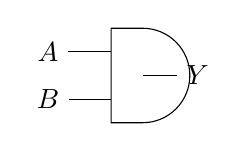
\begin{tikzpicture}[scale=1]
            % Simple custom AND gate to avoid reliance on gate shape anchors
            % Input nodes
            \node (A) at (-1,0.3) {$A$};
            \node (B) at (-1,-0.3) {$B$};
            % Wires to gate
            \draw (A.east) -- (-0.2,0.3);
            \draw (B.east) -- (-0.2,-0.3);
            % Gate body: rectangle on the left and semicircle on the right
            \draw (-0.2,0.6) -- (-0.2,-0.6) -- (0.2,-0.6) arc (-90:90:0.6) -- cycle;
            % Output
            \node (Y) at (0.9,0) {$Y$};
            \draw (0.6,0) -- (Y.west);
            \draw (0.2,0) -- (0.6,0);
        \end{tikzpicture}
    \end{center}    
\end{definition}

\begin{definition}[OR Gate]
    An OR gate outputs 1 if at least one input is 1. The truth table for a 2-input OR gate is shown in Table \ref{tab:or_gate}.
    \\
    The logic function for an OR gate with inputs $A$ and $B$ can be expressed as:
    $$
        L(A, B) = A + B
    $$
    The digital logic symbol for an OR gate is shown below:
    \begin{center}
        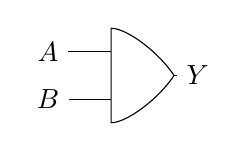
\begin{tikzpicture}[scale=1]
            % Simple custom OR gate to avoid reliance on gate shape anchors
            % Input nodes
            \node (A) at (-1,0.3) {$A$};
            \node (B) at (-1,-0.3) {$B$};
            % Wires to gate
            \draw (A.east) -- (-0.2,0.3);
            \draw (B.east) -- (-0.2,-0.3);
            % Gate body: curved shape
            \draw (-0.2,0.6) .. controls (0,0.6) and (0.4,0.3) .. (0.6,0) .. controls (0.4,-0.3) and (0,-0.6) .. (-0.2,-0.6) -- cycle;
            % Output
            \node (Y) at (0.9,0) {$Y$};
            \draw (0.6,0) -- (Y.west);
        \end{tikzpicture}
    \end{center}
\end{definition}    

\begin{definition}[NOT Gate]
    A NOT gate outputs the inverse of the input. The truth table for a NOT gate is shown in Table \ref{tab:not_gate}.
    \\
    The logic function for a NOT gate with input $A$ can be expressed as:
    $$
        L(A) = \overline{A}
    $$
    The digital logic symbol for a NOT gate is shown below:
    \begin{center}
        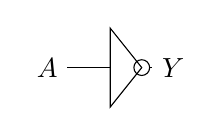
\begin{tikzpicture}[scale=1]
            % Input node
            \node (A) at (-1,0) {$A$};
            % Wire to gate
            \draw (A.east) -- (-0.2,0);
            % Gate body: triangle with circle at output
            \draw (-0.2,0.5) -- (0.2,0) -- (-0.2,-0.5) -- cycle;
            \draw (0.2,0) circle (0.1);
            % Output
            \node (Y) at (0.6,0) {$Y$};
            \draw (0.3,0) -- (Y.west);
        \end{tikzpicture}
    \end{center}
\end{definition}


\subsection{Additional Logic Gates}
\begin{example}[XOR Operation]
    We have two swtiches, when both switches are in the same state (both open or both closed), the output is 0. When the switches are in different states (one open and one closed), the output is 1. The truth table for this operation is shown below:
    \begin{table}[h!]
        \centering
        \begin{tabular}{|c|c|c|}      
            \hline
            $x_1$ & $x_2$ & $L(x_1, x_2)$ \\
            \hline
            0 & 0 & 0 \\
            0 & 1 & 1 \\
            1 & 0 & 1 \\
            1 & 1 & 0 \\
            \hline
        \end{tabular}
        \caption{Truth Table for XOR Operation}
        \label{tab:xor_gate}
    \end{table}
    \\
    The logic function can be expressed as:
    $$
        L(x_1, x_2) = x_1 \oplus x_2 = \overline{x_1}x_2 + x_1\overline{x_2}
    $$
    where $\oplus$ denotes the XOR operation.
\end{example}

\begin{definition}[XOR Gate]
    An XOR gate outputs 1 if the inputs are different. The truth table for a 2-input XOR gate is shown in Table \ref{tab:xor_gate}.
    \\
    The logic function for an XOR gate with inputs $A$ and $B$ can be expressed as:
    $$
        L(A, B) = A \oplus B = \overline{A}B + A\overline{B}
    $$
    where $\oplus$ denotes the XOR operation.
    The digital logic symbol for an XOR gate is shown below:
    \begin{center}
        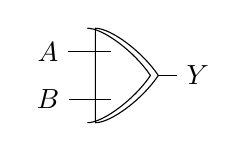
\begin{tikzpicture}[scale=1]
            % Input nodes
            \node (A) at (-1,0.3) {$A$};
            \node (B) at (-1,-0.3) {$B$};
            % Wires to gate
            \draw (A.east) -- (-0.2,0.3);
            \draw (B.east) -- (-0.2,-0.3);
            % Gate body: curved shape with extra curve on input side
            \draw (-0.4,0.6) .. controls (-0.2,0.6) and (0.2,0.3) .. (0.4,0) .. controls (0.2,-0.3) and (-0.2,-0.6) .. (-0.4,-0.6) -- cycle;
            \draw (-0.5,0.6) .. controls (-0.3,0.6) and (0.1,0.3) .. (0.3,0) .. controls (0.1,-0.3) and (-0.3,-0.6) .. (-0.5,-0.6);
            % Output
            \node (Y) at (0.9,0) {$Y$};
            \draw (0.4,0) -- (Y.west);
        \end{tikzpicture}
    \end{center}
\end{definition}


In addition, we have the following gates:
\begin{definition}[NAND Gate]
    A NAND gate outputs 0 only if all inputs are 1. The truth table for a 2-input NAND gate is shown in Table \ref{tab:nand_nor_gates}.
    \\
    The logic function for a NAND gate with inputs $A$ and $B$ can be expressed as:
    $$
        L(A, B) = \overline{A \cdot B} = \overline{A} + \overline{B}
    $$
    The digital logic symbol for a NAND gate is shown below:
    \begin{center}
        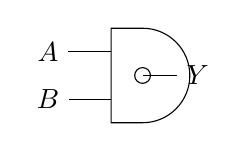
\begin{tikzpicture}[scale=1]
            % Input nodes
            \node (A) at (-1,0.3) {$A$};
            \node (B) at (-1,-0.3) {$B$};
            % Wires to gate
            \draw (A.east) -- (-0.2,0.3);
            \draw (B.east) -- (-0.2,-0.3);
            % Gate body: rectangle on the left and semicircle on the right with circle at output
            \draw (-0.2,0.6) -- (-0.2,-0.6) -- (0.2,-0.6) arc (-90:90:0.6) -- cycle;
            \draw (0.2,0) circle (0.1);
            % Output
            \node (Y) at (0.9,0) {$Y$};
            \draw (0.6,0) -- (Y.west);
            \draw (0.2,0) -- (0.6,0);
        \end{tikzpicture}
    \end{center}
\end{definition}

\begin{definition}
    
\end{definition}

\begin{shaded}
    \textbf{NAND and NOR Gates are Cheaper} NAND gates and NOR gates are cheaper than AND and OR gates because they require fewer transistors to implement. A 2-input NAND gate can be implemented using 4 transistors, while a 2-input AND gate requires 6 transistors (4 for the NAND gate and 2 for the NOT gate). The same applies to NOR and OR gates.

    \textbf{NAND and NOR Gates are Universal (Functionally Complete)} Additionally, NAND and NOR gates are universal gates, meaning that any logic function can be implemented using only NAND or NOR gates. 
    
    This makes them more versatile and cost-effective for building complex digital circuits.
\end{shaded}


\paragraph{Commonly Used Logic Operators} Below is a table summarizing the commonly used logic operators:
\begin{table}[h!]
    \centering
    \begin{tabular}{|c|c|c|}
        \hline
        Operator & Symbol & Description \\
        \hline
        AND & $\cdot$ or no symbol & Outputs 1 if all inputs are 1 \\
        OR & $+$ & Outputs 1 if at least one input is 1 \\
        NOT & $\overline{x}$ & Outputs the inverse of the input \\
        inverse & $'$ or $\sim$ & Outputs the 2's complement of the input \\
        XOR & $\oplus$ & Outputs 1 if inputs are different \\
        NAND & $\overline{\cdot}$ & Outputs 0 if all inputs are 1 \\
        NOR & $\overline{+}$ & Outputs 0 if at least one input is 1 \\
        XNOR & $\overline{\oplus}$ & Outputs 1 if inputs are the same \\
        \hline
    \end{tabular}
    \caption{Commonly Used Logic Operators}
\end{table}

\subsection{Sum of Products (SOP) Form}
\begin{definition}[Literal]
    A literal is a variable or its negation. For example, $A$ and $\overline{A}$ are literals.  A literal can be either true or false, and it represents a single value in a logical expression.

\end{definition}

\begin{definition}[Product Term]
    A product term is a logical synonym for AND.
\end{definition}

\begin{definition}[Sum Term]
    A sum term is a logical synonym for OR.
\end{definition}

\begin{definition}[Sum of Products (SOP) Form]
    A logical expression is in sum of products (SOP) form if it is a sum of product terms. For example, the expression $AB + \overline{A}C + BC$ is in SOP form.
\end{definition}

\begin{definition}[Minterm]
    A product term that evaluates to one for exactly one row of the truth table is called a minterm.
\end{definition}
\begin{example}[Minterm]
    For a given truth table for $x_1, x_2, x_3$, the minterms are:
    \begin{table}[h!]
        \centering
        \begin{tabular}{|c|c|c|c|}
            \hline
            $x_1$ & $x_2$ & $x_3$ & Minterm \\
            \hline
            0 & 0 & 0 & $m_0 = \overline{x_1}\overline{x_2}\overline{x_3}$ \\
            0 & 0 & 1 & $m_1 = \overline{x_1}\overline{x_2}x_3$ \\
            0 & 1 & 0 & $m_2 = \overline{x_1}x_2\overline{x_3}$ \\
            0 & 1 & 1 & $m_3 = \overline{x_1}x_2x_3$ \\
            1 & 0 & 0 & $m_4 = x_1\overline{x_2}\overline{x_3}$ \\
            1 & 0 & 1 & $m_5 = x_1\overline{x_2}x_3$ \\
            1 & 1 & 0 & $m_6 = x_1x_2\overline{x_3}$ \\
            1 & 1 & 1 & $m_7 = x_1x_2x_3$ \\
            \hline
        \end{tabular}
        \caption{Minterms for 3 Variables}
        \label{tab:minterms}

    \end{table}
    \\
    Note that each minterm corresponds to a unique combination of input values that produces an output of 1. To create the minterm, you would try to make every literal one.

\end{example}

\begin{definition}[Canonical SOP Form]
    A logical expression is in canonical SOP form if it is a sum of minterms. 
\end{definition}

\subsection{Product of Sums (POS) Form}

\begin{definition}[Product of Sums (POS) Form]
    A logical expression is in product of sums (POS) form if it is a product of sum terms. For example, the expression $(A + B)(\overline{A} + C)(B + C)$ is in POS form.
\end{definition}


\begin{definition}[Maxterm]
    A sum term that evaluates to zero for exactly one row of the truth table is called a maxterm.
\end{definition}

\begin{example}[Maxterm]
    For a given truth table for $x_1, x_2, x_3$, the maxterms are:
    \begin{table}[h!]
        \centering
        \begin{tabular}{|c|c|c|c|}
            \hline
            $x_1$ & $x_2$ & $x_3$ & Maxterm \\
            \hline
            0 & 0 & 0 & $M_0 = (x_1 + x_2 + x_3)$ \\
            0 & 0 & 1 & $M_1 = (x_1 + x_2 + \overline{x_3})$ \\
            0 & 1 & 0 & $M_2 = (x_1 + \overline{x_2} + x_3)$ \\
            0 & 1 & 1 & $M_3 = (x_1 + \overline{x_2} + \overline{x_3})$ \\
            1 & 0 & 0 & $M_4 = (\overline{x_1} + x_2 + x_3)$ \\
            1 & 0 & 1 & $M_5 = (\overline{x_1} + x_2 + \overline{x_3})$ \\
            1 & 1 & 0 & $M_6 = (\overline{x_1} + \overline{x_2} + x_3)$ \\
            1 & 1 & 1 & $M_7 = (\overline{x_1} + \overline{x_2} + \overline{x_3})$ \\
            \hline
        \end{tabular}
        \caption{Maxterms for 3 Variables}
        \label{tab:maxterms}
    \end{table}
    \\
    Note that each maxterm corresponds to a unique combination of input values that produces an output of 0. To create the maxterm, you would try to make every literal zero.
\end{example}

\begin{definition}[Canonical POS Form]
    A logical expression is in canonical POS form if it is a product of maxterms.
\end{definition}

\begin{theorem}[Converting between Canonical Forms]
    Any logical expression can be converted from canonical SOP form to canonical POS form and vice versa. For $i \in \{0, 1, \ldots, 2^n - 1\}$ and $S \subseteq \{0, 1, \ldots, 2^n - 1\}$, we have:
    \[
        f(x_1, x_2, \ldots, x_n) = \sum_{i \in S} m_i = \prod_{i \notin S} M_i
    \]
\end{theorem}
\begin{example}
    We have the following converison:
    $$
        f(x_1, x_2, x_3) = m_1 + m_3 + m_5 + m_7 = M_0 M_2 M_4 M_6
    $$
\end{example}

\subsection{Boolean Algebra and Logic Minimization}
\begin{definition}[Boolean Algebra]
    Boolean algebra is a branch of algebra that deals with binary variables and logical operations. It is a effective means to describe logic circuits with a set of rules derived from the axioms of Boolean algebra.
\end{definition}

\begin{definition}[Axioms of Boolean Algebra]
    The axioms of Boolean algebra are a set of fundamental rules that govern the behavior of binary variables and logical operations. The number stems consist only of the set $\{0, 1\}$, with the following axioms:
    \begin{itemize}
        \item $0 \cdot 0 = 0$
        \item $1 \cdot 1 = 1$
        \item $0 \cdot A = 0 \cdot 1 = 1 \cdot 0 = 0$ for any $A$
        \item if $x=0$ then $\overline{x} = 1$
    \end{itemize}

    \textbf{Dual Form} We can also derive the following logical equivalences from the axioms:
    \begin{itemize}
        \item $A + 0 = A$
        \item $A + 1 = 1$
        \item $0 + 1 = 1 + 0 = 1$
        \item $A + \overline{A} = 1$
    \end{itemize}

    where $1$ is the multiplicative identity and $0$ is the additive identity.
\end{definition}

\paragraph{Rules derived from the Axioms of Boolean Algebra} The following rules can be derived from the axioms of Boolean algebra:
\begin{theorem}
\begin{itemize}
    \item $x \cdot 0 = 0$ (Annihilation)
    \item $x \cdot 1 = 1 \cdot x = x$ (Identity)
    \item $x \cdot \overline{x} = 0$ (Complementation)
    \item $x \cdot x = x$ (Idempotent)
    \item $x + 0 = 0 + x = x$ (Identity)
    \item $x + 1 = 1 + x = 1$ (Annihilation)
    \item $x + \overline{x} = 1$ (Complementation)
\end{itemize}
\end{theorem}

\begin{theorem}
The following identities can be derived from the axioms of Boolean algebra:
\begin{itemize}
    \item Commutative Laws:
    \begin{itemize}
        \item $A + B = B + A$
        \item $A \cdot B = B \cdot A$
    \end{itemize}
    \item Associative Laws:
    \begin{itemize}
        \item $A + (B + C) = (A + B) + C$
        \item $A \cdot (B \cdot C) = (A \cdot B) \cdot C$
    \end{itemize}
    \item Distributive Laws:
    \begin{itemize}
        \item $A \cdot (B + C) = A \cdot B + A \cdot C$
        \item $A + (B \cdot C) = (A + B) \cdot (A + C)$
    \end{itemize}
\end{itemize}
\end{theorem}
\begin{proof}
    By perfect induction. We can exhaustively check all possible values of $A$, $B$, and $C$ (0 or 1) to verify that both sides of each identity yield the same result.
\end{proof}

\begin{theorem}[Covering Theorem]
     The following is true:
    $$    
    x + xy = x
    $$
    and its dual:
    $$
    x(x + y) = x
    $$
\end{theorem}

\begin{theorem}[Combining Theorem]
    The following is true:
    $$
    xy + x\overline{y} = x
    $$
    and its dual:
    $$
    (x + y)(x + \overline{y}) = x
    $$
    
\end{theorem}

\begin{theorem}[De Morgan's Theorem]
    The following is true:
    $$
    \overline{xy} = \overline{x} + \overline{y}
    $$
    and its dual:
    $$
    \overline{x + y} = \overline{x} \cdot \overline{y}
    $$
\end{theorem}
\begin{proof}
    By direct proof. We have:
    \begin{align*}
        \overline{xy} &= \overline{x}\overline{y} + \overline{x}y + x\overline{y} \quad (\text{In Canonical SOP Form}) \\
        &= \overline{x}\overline{y} + \overline{x}y + x\overline{y} + x\overline{y} \quad (\text{Adding } x\overline{y} \text{ using $x + x = x$}) \\
        &= \overline{x}(\overline{y} + y) + \overline{y}(x + \overline{x}) \quad (\text{Using Distributive Law}) \\
        &= \overline{x} \cdot 1 + \overline{y} \cdot 1 \quad (\text{Using Complementation}) \\
        &= \overline{x} + \overline{y} \quad (\text{Using Identity})
    \end{align*}
\end{proof}

\begin{theorem}[Absorption / Redundancy Theorem]
    The following is true:
    $$
    x + \overline{x}y = x + y
    $$
    and its dual:
    $$
    x(\overline{x} + y) = xy
    $$
\end{theorem}
\begin{proof}
    By direct proof. We have:
    \begin{align*}
        x + \overline{x}y &= x + \overline{x}y + xy \quad (\text{Adding } xy \text{ using } x + xy = x) \\
        &= x(1 + y) + \overline{x}y \quad (\text{Using Distributive Law}) \\
        &= x \cdot 1 + \overline{x}y \quad (\text{Using Identity}) \\
        &= x + y \quad (\text{Using Combining Theorem})
    \end{align*}
\end{proof}

\begin{shaded}
    \textbf{Logic Minimization} The goal of logic minimization is to reduce the number of logic gates and inputs in a digital circuit while maintaining its functionality. This is important because it can lead to cost savings, improved performance, and reduced power consumption. Logic minimization can be achieved through various techniques, including Boolean algebra simplification, Karnaugh maps, and the Quine-McCluskey algorithm.
\end{shaded}

\begin{theorem}[Nand as SOP]
    And SOP circuit can be implemented using only NAND gates.
\end{theorem}

\begin{theorem}[Nor as POS]
    A POS circuit can be implemented using only NOR gates.
\end{theorem}

\begin{example}[Gumball Fact]
    Consider three sensors $s_0, s_1, s_2$ that detect defects in Gumballs. Those sensors are normally 0, but would be 1 if a defect is detected as follows:
    $$
        \begin{cases}
            s_0 = 1 & \text{if the Gumball is too small} \\
            s_1 = 1 & \text{if the Gumball is too big} \\
            s_2 = 1 & \text{if the Gumball is too light}
        \end{cases}
    $$
    We are to design a circuit that would output 1 if the Gumball is either too large or too small and too light. We can express canonical SOP form as:
    \begin{align*}
        L(s_0, s_1, s_2) &= m_3 + m_4 + m_5 + m_6 + m_7 = \overline{s_0}s_1s_2 + s_2\overline{s_0}\overline{s_2} + s_0\overline{s_1}s_2 + s_0s_1\overline{s_2} + s_0s_1s_2 \\
        \intertext{Using the Combining Theorem}
        &= \overline{s_0}s_1s_2 + s_2\overline{s_0}\overline{s_2} + s_0s_2 + s_0s_1 \\
        \intertext{Using the Absorption Theorem}
        &= s_2\overline{s_0} + s_0s_2 + s_0s_1 \\
        \intertext{Using the Covering Theorem}
        &= s_2 + s_0s_1 
    \end{align*}
\end{example}
\section{Digital Storage Elements}

\section{Finite State Machines (FSM)}

\chapter{Computer Organization and Assembly Language}
\begin{shaded}
\textbf{What is Assembly Language?} We know that we can run C/C++ on any computer (Machine Agnostic), but how does the computer understand C/C++? The answer is the compiler that parse it to assembly through:

\begin{enumerate}
    \item \textbf{Front-end Parser:} The front-end parser would parse the C/C++ code into an intermediate representation (IR), which is a low-level representation of the code that is easier to optimize. The front-end parser would also perform optimizations on the IR, such as loop unrolling, inlining, and dead code elimination.
    \item \textbf{Back-end Parser:} The back-end parser would take the optimized IR and generate assembly code for a specific architectures.
\end{enumerate}
\end{shaded}
The assembly code is then assembled into machine code, which is a series of 0s and 1s that the computer can understand. The assembly would be specific to the architecture of the computer (machine dependent), which is why we have different assembly languages for different architectures (e.g., x86, RISC-V, ARM).
\section{Computer Organization}

\section{Assembly Language}
\end{document}

